%! Author = taj
%! Date = 7/22/25

% Preamble
\documentclass[11pt]{article}

% Packages
\usepackage{amsmath}
\usepackage{graphicx}
\usepackage{float}
\usepackage{upgreek}

\title{12. Temperaturno raztezanje snovi}
\author{Taj Šobot}

% Document
\begin{document}
    \maketitle
    \flushleft

    Pri tej vaji smo merili kako se snovi raztezajo ko jih segrevamo.

    \section{Meritve}
    Skozi aluminijasto cev smo vlivali vodo.
    Cev je imela dolžino
    \[
        l_0 = (35.7 \pm 0.1) cm
    \]
    Sledijo meritve po vlitju vode:

    \begin{table}[h!]
        \centering
        \begin{tabular}{|c|c|}
            \hline
            $T [^\circ C]$ & $\Delta l [mm] $ \\
            \hline
            22 & 0.02  \\
            42 & 0.13  \\
            60 & 0.27  \\
            80 & 0.41  \\
            92 & 0.5   \\
            \hline
        \end{tabular}
        \caption{tabela}
        \label{tab:1}
    \end{table}

    V drugem delu vaje smo pa merili temperaturni raztezek tekočin.
    Spodaj so meritve za vodo in alkohol:
    \begin{table}[h!]
        \centering
        \begin{tabular}{|c|c|c|}
            \hline
            $T [^\circ C]$ & $\Delta l [mm] (voda)$ & $\Delta l [mm] (alkohol)$ \\
            \hline
            25 & 11.8 &  7.4 \\
            28 & 15.0 & 16.2 \\
            31 & 16.2 & 23.0 \\
            34 & 17.0 & 28.8 \\
            37 & 19.7 & 34.7 \\
            40 & 21.6 &      \\
            43 & 24.2 &      \\
            46 & 27.1 &      \\
            49 & 29.9 &      \\
            52 & 32.4 &      \\
            \hline
        \end{tabular}
        \caption{tabela}
        \label{tab:2}
    \end{table}
    Meritve manjkajo ker je alkohol začel naraščati preko posode.
    \\
    Začetni volumen je bil:
    \[
        V_{h2o} = (215 \pm 5) ml
    \]
    in
    \[
        V_{alk} = (130 \pm 5) ml
    \]

    \section{Rezultati}

    Lineariziran garaf za enačbo:
    \[
        \delta L = L_0 \alpha \Delta T
    \]
    \begin{figure}[H]
        \centering
        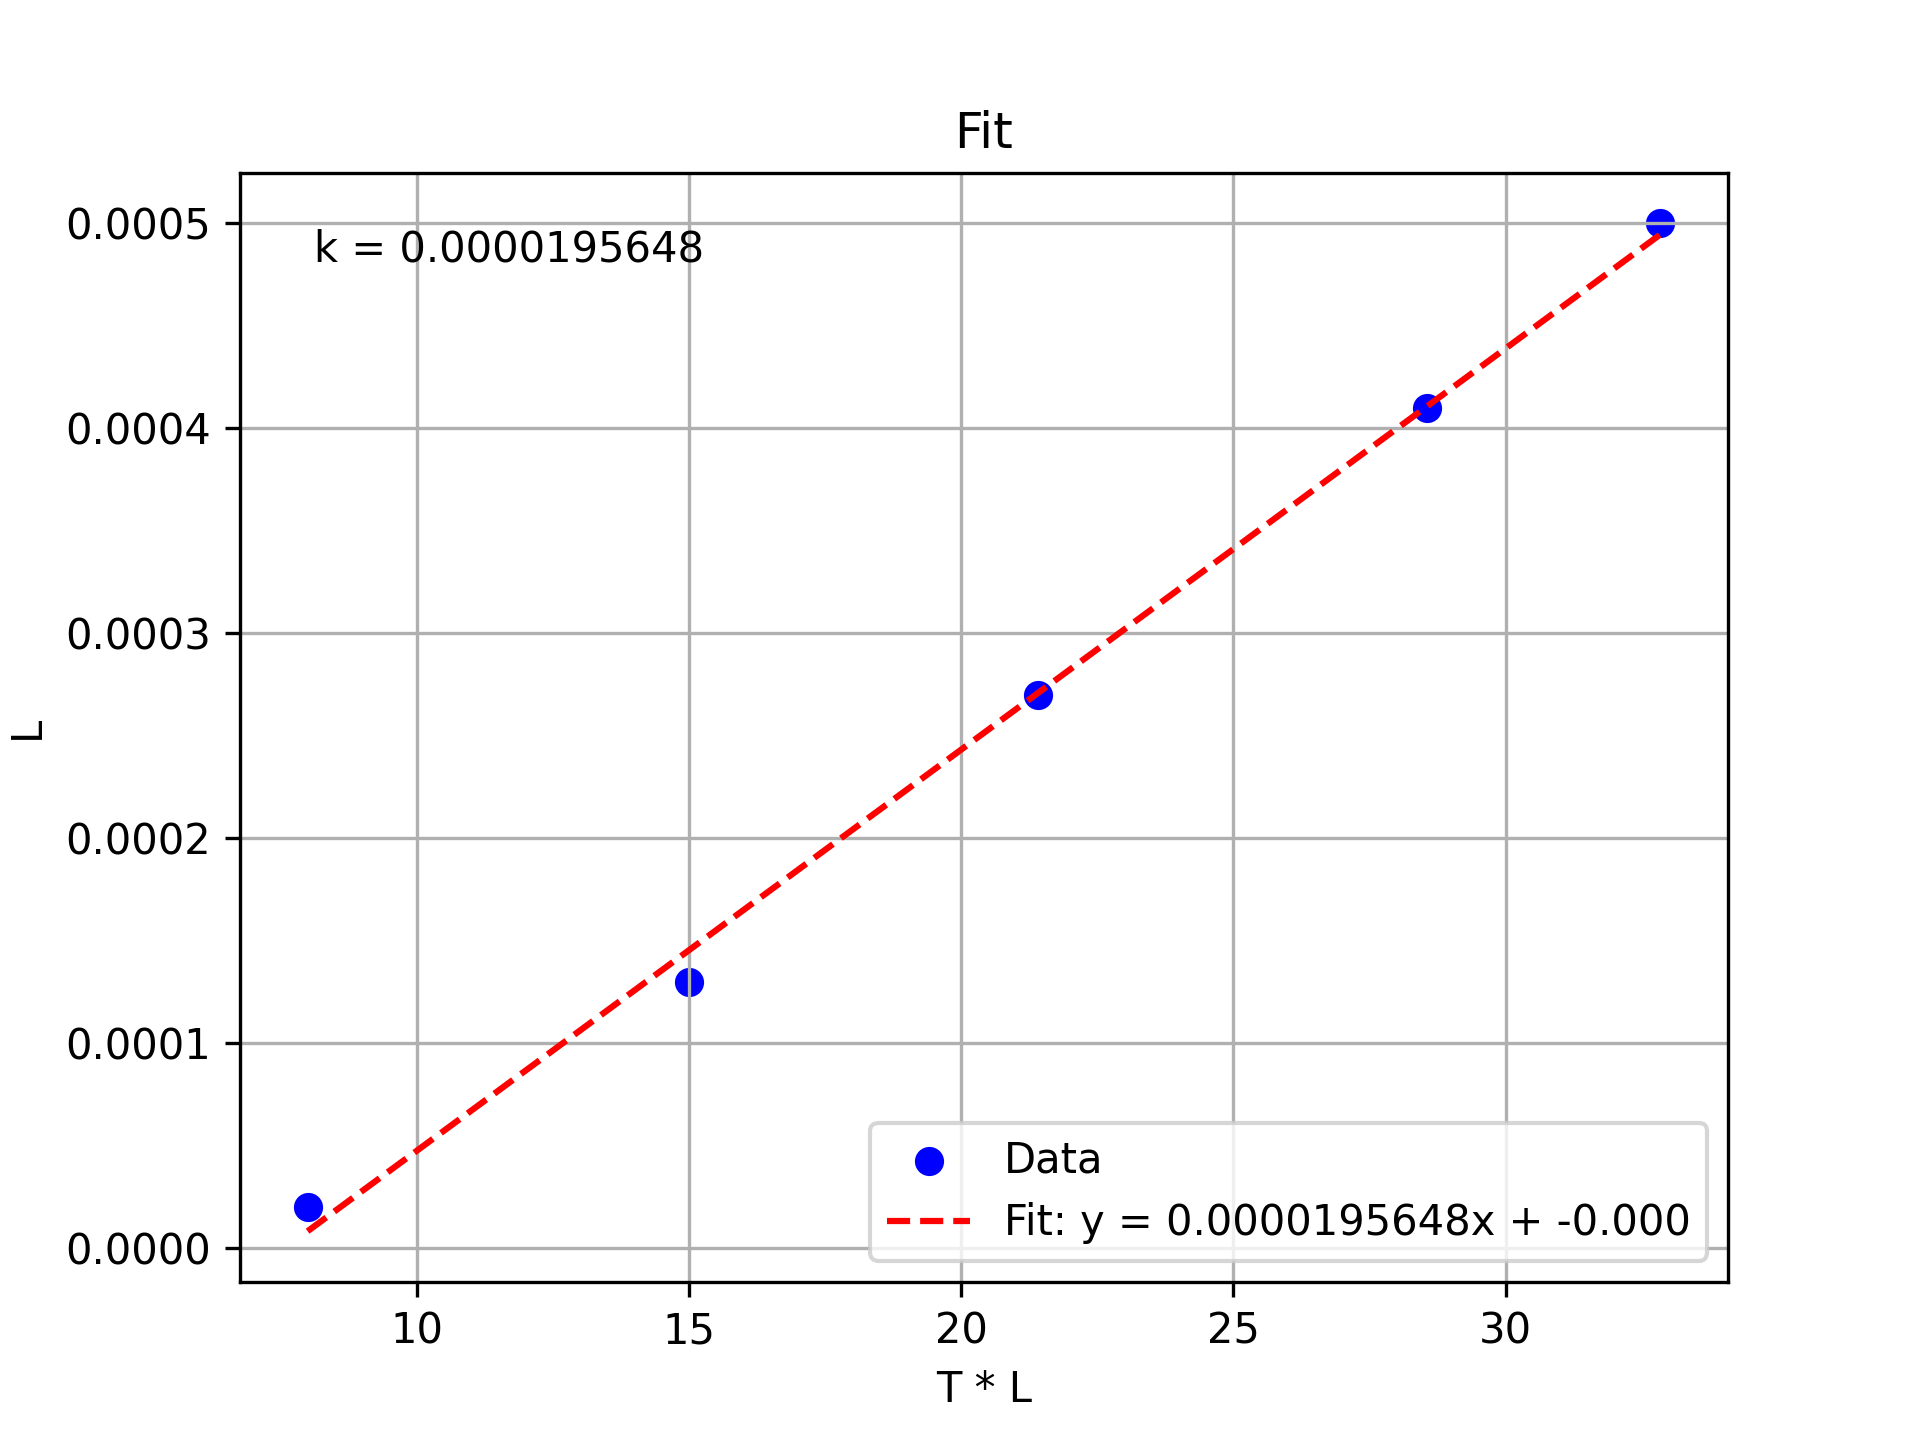
\includegraphics[width=0.9\textwidth]{graf}
        \caption{Graf1}
        \label{fig:3}
    \end{figure}
    Iz grafa odčitamo konstantni člen dobimo:
    \[
        \alpha = (1.9 \pm 0.1)*10^{-5} \frac{1}{K}
    \]
    Ta rezultat je realen za aluminij.

    Drugi del vaje pa smo morali izračunat volumski raztezek tekočin:
    Voda:
    \begin{figure}[H]
        \centering
        
\includegraphics[width=0.9\textwidth]{graf2}
        \caption{Graf2}
        \label{fig:4}
    \end{figure}
    \[
        k_v = (0.006 \pm 0.0004) m^3/K
    \]
    Torej:
    \[
        \beta_{vode} = k_v / V_{vode} = (0.055 \pm 0.03) 1/K
    \]
    Še alkohol:
    \begin{figure}[H]
        \centering
        
\includegraphics[width=0.9\textwidth]{graf3}
        \caption{Graf3}
        \label{fig:7}
    \end{figure}
    \[
        k_a = (0.022 \pm 0.0002) m^3/K
    \]
    Torej:
    \[
        \beta_{alk} = k_a / V_{alk} = (0.0011 \pm 0.03) 1/K
    \]


\end{document}